\begin{opinion}
\textbf{Opinión de los tutores del Trabajo Diploma titulado “TkHURSv1.1: SOFTWARE ESTADÍSTICO PARA CALCULAR LOS PERÍODOS DE RETORNO DE HURACANES” del estudiante Yasmany David Morejón Cruz.}\\


El trabajo de tesis desarrollado por el estudiante Yasmany David Morejón Cruz de Ciencia de la Computación aborda un tema de suma importancia como son los ciclones tropicales. La actualización el software TkHURS para el análisis de períodos de retorno a través de un Modelo de Poisson utilizando la cronología de Ciclones Tropicales en Cuba se desarrolló con el objetivo de realizar investigaciones para la prevención de estos fenómenos. Este comprende los aspectos matemáticos necesarios para realizar el análisis primario de datos que incluyan los diferentes métodos.\\


El estudiante se enfrentó al trabajo con independencia, no logró solucionar todo el problema planteado debido a los inconvenientes presentados en este período por la situación de la Covid19 y dejando claro que todas las discusiones fueron a través del teléfono fijo y WhatsApp. A pesar de todo para lograr los objetivos propuestos el estudiante necesitó hacer uso de los conocimientos recibidos en la carrera y tuvo que ver temas relacionados con la estadística y la climatología.

\begin{figure}[H]
\centering
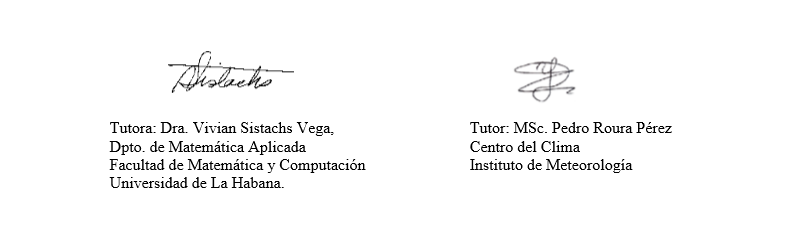
\includegraphics[scale=0.6]{firmas_tutores}
\end{figure}


\end{opinion}